\begin{block}{Partitions interactives}
\begin{figure}
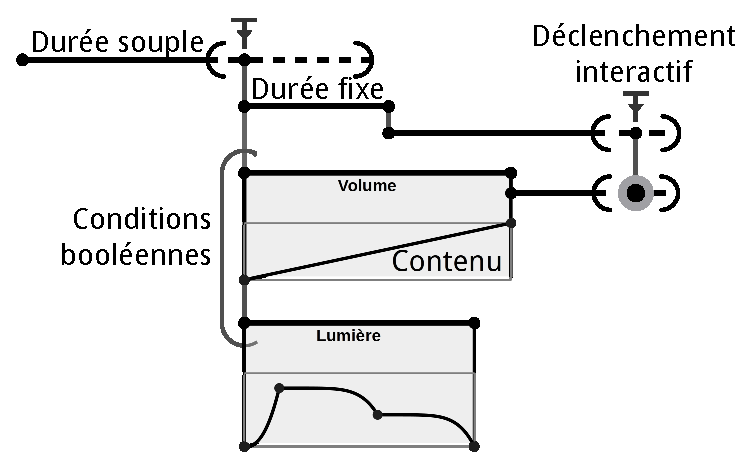
\includegraphics[width=\columnwidth]{images/score.eps}
\caption{Syntaxe d'une partition interactive}
\end{figure}
Possibilités d'écritures forment un langage de programmation structuré axé sur l'organisation temporelle. Possèe la notion de boucles et de hiérarchie, 
mais pas de calcul.
Applications : musique interactive, scénographie et spectacle vivant, contrôle de robots.
Autres approches graphiques : Antescofo, INscore, OpenMusic; ainsi qu'approches programmatiques : Abjad, Tuiles réactives, \dots
\end{block}